%%%%%%%%%%%%%%%%%%%%%%%%%%%%%%%%%%%%%%%%%%%%%%%%%%%%%%%%%%%%%%%%%%%%%
\subsection{Increasing Pipeline Parallelism by Repartitioning Memories (8 marks)}
%%%%%%%%%%%%%%%%%%%%%%%%%%%%%%%%%%%%%%%%%%%%%%%%%%%%%%%%%%%%%%%%%%%%%

The work in this section is based on L2 pipelining with T2P memory.

\begin{table}
    \caption{Performance and utilization estimates for \texttt{mmult\_float}}\label{tab:float-summary}
    {
\small
\centering
\begin{tabularx}{\textwidth}{cl*{6}{R}C}
    \toprule

    \multicolumn{2}{c}{\multirow{2}{*}{Profile}} &
    \multicolumn{2}{c}{Latency (cycles)}         &
    \multicolumn{2}{c}{Latency (ms)}             &
    \multicolumn{2}{c}{Interval (cycles)}        &
    \multicolumn{1}{c}{\multirow{2}{*}{\makecell*{Pipeline
                \\ Type}}}                                                                                                                \\

    \cmidrule(lr){3-4}
    \cmidrule(lr){5-6}
    \cmidrule(lr){7-8}
                                                 &
                                                 &
    \multicolumn{1}{c}{min}                      &
    \multicolumn{1}{c}{max}                      &
    \multicolumn{1}{c}{min}                      &
    \multicolumn{1}{c}{max}                      &
    \multicolumn{1}{c}{min}                      &
    \multicolumn{1}{c}{max}                      & \\
    \midrule
    \ref{sec:1a}                      & Baseline (AutoPipe) & 85160 & 85160 & 1.236 & 1.236 & 85161 & 85161 & none \\
\rowcolor{rowhlt}\ref{sec:1a}       & Baseline (NoPipe) & 228022 & 228022 & 2.280 & 2.280 & 228023 & 228023 & none \\
\ref{sec:1bL3}                          & L3 Pipelining & 85286 & 85286 & 1.238 & 1.238 & 85287 & 85287 & none \\
\ref{sec:1bL2}                     & L2 Pipelining (1WnR) & 7341 & 7341 & 0.073 & 0.073 & 7342 & 7342 & none \\
\ref{sec:1bL2}                     & L2 Pipelining (T2P) & 13885 & 13885 & 0.139 & 0.139 & 13886 & 13886 & none \\
\ref{sec:1bL1}                     & L1 Pipelining (1WnR) & 6193 & 6193 & 0.062 & 0.062 & 6194 & 6194 & none \\
\ref{sec:1bL1}                      & L1 Pipelining (T2P) & 5953 & 5953 & 0.060 & 0.060 & 5954 & 5954 & none \\
\rowcolor{rowhlt}\ref{sec:1c}  & Baseline (L2, AutoPipe, T2P) & 13759 & 13759 & 0.138 & 0.138 & 13760 & 13760 & none \\
\ref{sec:1cDim}                     & Partition (\texttt{dim}=1, \texttt{factor}=2) & 13772 & 13772 & 0.138 & 0.138 & 13773 & 13773 & none \\
\rowcolor{rowhlt}\ref{sec:1cDim}    & Partition (\texttt{dim}=2, \texttt{factor}=2) & 8703 & 8703 & 0.087 & 0.087 & 8704 & 8704 & none \\
\ref{sec:1cFac}                     & Partition (\texttt{dim}=2, \texttt{factor}=4) & 6175 & 6175 & 0.062 & 0.062 & 6176 & 6176 & none \\
\ref{sec:1cFac}                     & Partition (\texttt{dim}=2, \texttt{factor}=8) & 4911 & 4911 & 0.049 & 0.049 & 4912 & 4912 & none \\
\rowcolor{rowhlt}\ref{sec:1cFac}   & Partition (\texttt{dim}=2, \texttt{factor}=16) & 4279 & 4279 & 0.043 & 0.043 & 4280 & 4280 & none \\
\ref{sec:1cFac}                    & Partition (\texttt{dim}=2, \texttt{factor}=32) & 3963 & 3963 & 0.040 & 0.040 & 3964 & 3964 & none \\
    \bottomrule
\end{tabularx}

\begin{tabularx}{\textwidth}{cl*{5}{c}*{2}{C}}
    \toprule

    \multicolumn{2}{c}{\multirow{2}{*}{Profile}} &
    \multicolumn{5}{c}{Utilization Summary}      &
    \multicolumn{2}{c}{Instance}                   \\

    \cmidrule(lr){3-7}
    \cmidrule(lr){8-9}
                                                 &
                                                 &
    \multicolumn{1}{c}{BRAM\_18K}                &
    \multicolumn{1}{c}{DSP}                      &
    \multicolumn{1}{c}{FF}                       &
    \multicolumn{1}{c}{LUT}                      &
    \multicolumn{1}{c}{URAM}                     &
    \multicolumn{1}{c}{fadd}                     &
    \multicolumn{1}{c}{fmul}                       \\

    \midrule
    \ref{sec:1a}                      & Baseline (AutoPipe) & 13 (4\%) & 5 (2\%) & 1050 (\textasciitilde 0\%) & 2000 (3\%) & 0 (0\%) & 1 & 1 \\
\rowcolor{rowhlt}\ref{sec:1a}       & Baseline (NoPipe) & 14 (5\%) & 5 (2\%) & 817 (\textasciitilde 0\%) & 1635 (3\%) & 0 (0\%) & 1 & 1 \\
\ref{sec:1bL3}                          & L3 Pipelining & 14 (5\%) & 5 (2\%) & 921 (\textasciitilde 0\%) & 1713 (3\%) & 0 (0\%) & 1 & 1 \\
\ref{sec:1bL2}                     & L2 Pipelining (1WnR) & 182 (65\%) & 80 (36\%) & 38357 (36\%) & 34359 (64\%) & 0 (0\%) & 16 & 16 \\
\ref{sec:1bL2}                     & L2 Pipelining (T2P) & 16 (5\%) & 10 (4\%) & 24710 (23\%) & 22359 (42\%) & 0 (0\%) & 2 & 2 \\
\ref{sec:1bL1}                     & L1 Pipelining (1WnR) & 70 (25\%) & 800 (363\%) & 415044 (390\%) & 243128 (457\%) & 0 (0\%) & 160 & 160 \\
\ref{sec:1bL1}                      & L1 Pipelining (T2P) & 16 (5\%) & 100 (45\%) & 312992 (294\%) & 120185 (225\%) & 0 (0\%) & 20 & 20 \\
\rowcolor{rowhlt}\ref{sec:1c}  & Baseline (L2, AutoPipe, T2P) & 16 (5\%) & 10 (4\%) & 24776 (23\%) & 22615 (42\%) & 0 (0\%) & 2 & 2 \\
\ref{sec:1cDim}                     & Partition (\texttt{dim}=1, \texttt{factor}=2) & 16 (5\%) & 10 (4\%) & 32491 (30\%) & 45788 (86\%) & 0 (0\%) & 2 & 2 \\
\rowcolor{rowhlt}\ref{sec:1cDim}    & Partition (\texttt{dim}=2, \texttt{factor}=2) & 16 (5\%) & 20 (9\%) & 27306 (25\%) & 19326 (36\%) & 0 (0\%) & 4 & 4 \\
\ref{sec:1cFac}                     & Partition (\texttt{dim}=2, \texttt{factor}=4) & 20 (7\%) & 40 (18\%) & 31022 (29\%) & 20786 (39\%) & 0 (0\%) & 8 & 8 \\
\ref{sec:1cFac}                     & Partition (\texttt{dim}=2, \texttt{factor}=8) & 36 (12\%) & 80 (36\%) & 37606 (35\%) & 26782 (50\%) & 0 (0\%) & 16 & 16 \\
\rowcolor{rowhlt}\ref{sec:1cFac}   & Partition (\texttt{dim}=2, \texttt{factor}=16) & 68 (24\%) & 160 (72\%) & 52606 (49\%) & 40402 (75\%) & 0 (0\%) & 32 & 32 \\
\ref{sec:1cFac}                    & Partition (\texttt{dim}=2, \texttt{factor}=32) & 132 (47\%) & 320 (145\%) & 72201 (67\%) & 65294 (122\%) & 0 (0\%) & 64 & 64 \\
    \bottomrule
\end{tabularx}
}

\begin{enumerate}[nosep]
    \footnotesize
    \item ``\{L1, L2, L3\} Pipelining'' are based on Baseline (NoPipe).
    \item ``L2/Partition'' are based on L2 Pipelining.
\end{enumerate}
\end{table}

%%%%%%%%%%%%%%%%%%%%%%%%%%%%%%%%%%%%%%%%%%%%%%%%%%%%%%%%%%%%%%%%%%%%%
\subsubsection{Understanding the \texttt{dim} parameter}\label{sec:1cDim}

Instead of looking into the factor, which is of interest in this project,
we try to choose an appropriate \texttt{dim}.
The \texttt{dim} option is used to specify which dimension is partitioned.
\autoref{fig:float-partition-dim} is a figure coming from \textit{Vitis HLS User Guide (ug1399)}, which clearly shows the idea of \texttt{dim}.
In our application, the loop body of L2 is pipelined, which reads 256 elements from \texttt{in\_buf} and 256 elements from \texttt{weight\_buf}.
In order to improve parallelism, it is obvious that we should distribute the one vector of 256 elements to several blocks of memory.
That is, we need to set \texttt{dim} to 2.

\begin{figure}[ht!]
    \centering
    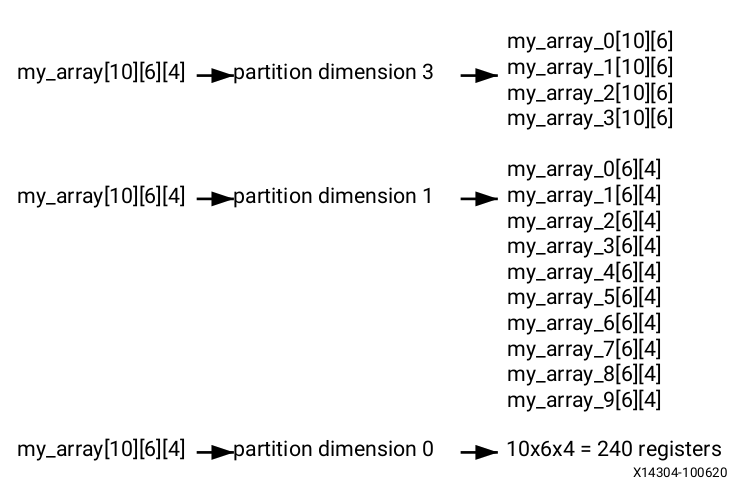
\includegraphics[scale=0.5]{images/float-partition-dim.png}
    \caption{Partitioning Array Dimensions}
    \label{fig:float-partition-dim}
\end{figure}

\begin{figure}[ht!]
    % \centering
    \begin{subfigure}[b]{\textwidth}
        \inputminted[firstline=3]{diff}{program/05-partition-d1-f2.diff}
        \caption{Setting array partition with \texttt{dim}=1}
        \label{fig:05-partition-d1-f2.diff}
    \end{subfigure}
    \begin{subfigure}[b]{\textwidth}
        \inputminted[firstline=3]{diff}{program/05-partition-d2-f2.diff}
        \caption{Setting array partition with \texttt{dim}=2}
        \label{fig:05-partition-d2-f2.diff}
    \end{subfigure}
    \caption{Comparing different setting of \texttt{dim}}\label{fig:05-partition-d12}
\end{figure}

I have also experimented on this, where the code is modified as \autoref{fig:05-partition-d12}.
The HLS summary (\autoref{tab:float-summary}) shows setting \texttt{dim} to 1 introduces more resource usage but the latency is worse.
On the contrary, setting \texttt{dim} to 2 leads to introducing more floating-point adders and multipliers and achieves a lower latency.
The result also supports our conclusion above.

%%%%%%%%%%%%%%%%%%%%%%%%%%%%%%%%%%%%%%%%%%%%%%%%%%%%%%%%%%%%%%%%%%%%%
\subsubsection{Trying different \texttt{factor}s}\label{sec:1cFac}

As shown in \autoref{tab:float-summary}, adding the \texttt{factor} to 32 makes the utilization of DSP and LUT exceeds the resource budget.
When \texttt{factor}=16, the latency is reduced to 9013, which means 25.3x improvement.
In this design, 32 floating point adders and 32 floating point multipliers are used, which is 16 times of that when array partition is not used.
From \autoref{tab:float-loop-06-partition-d2-f16}, it can be seen that the initiation interval is 8 cycles.

\begin{table}[ht!]
    \caption{Loop details for partition with \texttt{dim}=2 \texttt{factor}=16}
    \label{tab:float-loop-06-partition-d2-f16}
    \centering
    \begin{tabularx}{\textwidth}{ p{4cm} *{7}{C}}
    \toprule
    \multicolumn{1}{c}{\multirow{2}{*}{Loop Name}} &
    \multicolumn{2}{c}{Latency (cycles)}           &
    \multicolumn{1}{c}{\multirow{2}{*}{\makecell*{Iteration \\
    Latency}}}                                     &
    \multicolumn{2}{c}{Initiation Interval}        &
    \multicolumn{1}{c}{\multirow{2}{*}{\makecell*{Trip      \\
    Count}}}                                       &
    \multicolumn{1}{c}{\multirow{2}{*}{Pipelined}}          \\

    \cmidrule(lr){2-3}
    \cmidrule(lr){5-6}

                                                   &
    \multicolumn{1}{c}{min}                        &
    \multicolumn{1}{c}{max}                        &
                                                   &
    \multicolumn{1}{c}{achieved}                   &
    \multicolumn{1}{c}{target}                     &        \\
    \midrule
    \texttt{- LOAD\_OFF\_1} & 5 & 5 & 1 & - & - & 5 & no \\
\texttt{- LOAD\_W\_1} & 3860 & 3860 & 386 & - & - & 10 & no \\
\texttt{ + LOAD\_W\_2} & 384 & 384 & 3 & - & - & 128 & no \\
\texttt{- LOAD\_I\_1} & 3088 & 3088 & 386 & - & - & 8 & no \\
\texttt{ + LOAD\_I\_2} & 384 & 384 & 3 & - & - & 128 & no \\
\texttt{- L1\_L2} & 1918 & 1918 & 1287 & 8 & 1 & 80 & yes \\
\texttt{- STORE\_O\_1} & 136 & 136 & 17 & - & - & 8 & no \\
\texttt{ + STORE\_O\_2} & 15 & 15 & 3 & - & - & 5 & no \\
    \bottomrule
\end{tabularx}

\end{table}
